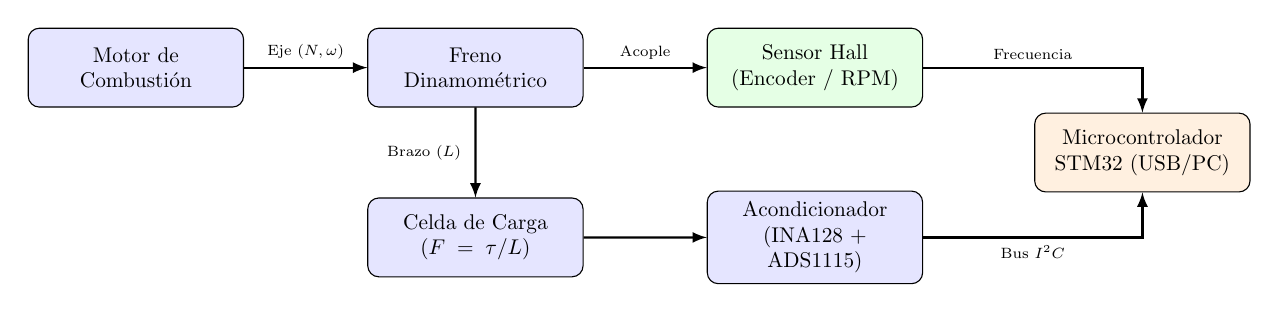
\begin{tikzpicture}[scale=0.77, transform shape,
    block/.style={rectangle, draw, fill=blue!10, text width=3.2cm, text centered,
                  rounded corners, minimum height=1.3cm, inner sep=5pt},
    line/.style={draw, -latex, thick}]

    \node [block] (motor) at (0, 0) {Motor de\\Combustión};
    \node [block] (freno) at (5.6, 0) {Freno\\Dinamométrico};
    \node [block, fill=green!10] (rpm) at (11.2, 0) {Sensor Hall\\(Encoder / RPM)};

    \node [block] (celda) at (5.6, -2.8) {Celda de Carga\\($F = \tau / L$)};
    \node [block] (acond) at (11.2, -2.8) {Acondicionador\\(INA128 + ADS1115)};
    \node [block, fill=orange!12] (mcu)   at (16.6, -1.4) {Microcontrolador\\STM32 (USB/PC)};

    \path [line] (motor) -- node[above, midway, font=\scriptsize] {Eje ($N, \omega$)} (freno);
    \path [line] (freno) -- node[above, midway, font=\scriptsize] {Acople} (rpm);
    \path [line] (freno) -- node[left=3pt, midway, font=\scriptsize] {Brazo ($L$)} (celda);
    \path [line] (celda) -- (acond);
    \path [line] (rpm.east) -- node[above, midway, font=\scriptsize] {Frecuencia} (rpm.east -| mcu.north) -- (mcu.north);
    \path [line] (acond.east) -- node[below, midway, font=\scriptsize] {Bus $\text{I}^2\text{C}$} (acond.east -| mcu.south) -- (mcu.south);
\end{tikzpicture}

